\chapter{System Setup}\label{ch:system-setup}

The \gls{sdh}~\cite{shadow-dex-hand} is a sophisticated robotic hand with a wide range of sensory feedback capabilities. To develop and test algorithms for this complex system, simulation is an invaluable tool. In this chapter, the practical setup of the project is presented, which involves simulating the \gls{sdh} within the dynamic simulator, Gazebo~\cite{gazebo}. \medskip

This simulation is based on the Shadow Robot Company's~\cite{shadow-robotics} \gls{ros}~\cite{ros} packages~\cite{shadow-ros-packages}, which provide a flexible and customizable framework for controlling the hand. This project uses Gazebo, a popular robot simulation environment, to simulate the physics of the hand and its interaction with the environment. To ensure reproducibility and portability, the development framework which encapsulates the simulation environment is built within a Docker container, which allows for easily distributing the code and dependencies to other researchers. Simulating the system additionally enables \gls{gt} values to be easily available, and safety is less of a concern, as a broken simulated hand, and additional equipment including sensors cost are potentially easier available in the form of simulated sensor inputs. \medskip

This simulation is based on the \gls{ros} packages developed by the Shadow Robot Company~\cite{shadow-robotics, ros, shadow-ros-packages}. These packages offer a flexible and customizable framework for controlling the hand. The simulation utilizes Gazebo, a widely-used robot simulation environment, to accurately model the hand's physics and its interactions with the environment. To ensure reproducibility and ease of distribution, the development framework, including the simulation environment, is encapsulated within a Docker container. This containerized approach allows for seamless sharing of the code and its dependencies with other researchers, promoting collaboration and portability. \medskip

Simulating the system provides the added benefit of readily accessible \gls{gt} values, ensuring accurate analysis and evaluation of algorithms. Moreover, safety concerns are mitigated in the simulation as the risk of damaging physical hardware or incurring additional costs for equipment and sensors is eliminated. Instead, these aspects can be readily simulated through virtual sensor inputs and virtual components. \medskip

In this chapter, a detailed description of the hardware and software used in this project's simulation setup is provided, which includes the software architecture of the simulation, including the \gls{ros} packages and Gazebo setup.

\section{Simulation Setup}\label{sec:system-setup-simulation-setup}

The \gls{cad} model of the \gls{sdh} is a highly detailed and accurate representation of the physical hand. The model is based on the original design of the real-world hand, which was developed by the Shadow Robot Company. The \gls{cad} model includes precise geometry for all of the hand's components, including the finger joints, tendons, and simple tactile sensors. The model also includes detailed material properties for each component, which are used to simulate the hand's physical behavior in the simulation.\medskip

The \gls{sdh}'s joints are labeled based on joint location according to~\appref{app:joint-abbreviations} and placement from the fingertip i.e. the outermost joint on the middle finger is labeled \texttt{MF1} while the innermost is \texttt{MF4}. The wrist joints are labeled \texttt{WR1} and \texttt{WR2}, where \texttt{WR1} is responsible for the hand's yaw and \texttt{WR2} is responsible for the hand's pitch rotation. \medskip

The structure of the hand can be seen in \figref{fig:robot-hand-skeleton} compared to a human hand in \figref{fig:human-hand-skeleton}. Here each joint is marked with a color, labeling the \gls{dof} for that particular joint. The red labels refer to joints with \num{1} \gls{dof}, blue refers to joints with a \gls{dof} equal to \num{2} and purple refers to two joints that are coupled. The coupling between joints is such that, a flexion of joint \num{1} imposes a constraint on joint \num{2}. If joint \num{1} exceeds a certain angle, it enforces joint \num{2} to flex accordingly to maintain the established constraint. Both joints are mechanically linked to a single motor, functioning as a combined joint denoted as joint \num{0} for control purposes. \medskip

As seen here the \gls{sdh} provides human-like dexterity due to its similar kinematics, see~\figref{app:human-and-robot-hand-kinematics}, and the comparable \gls{rom} of each joint, see~\tabref{app:range-of-motion-shadow-hand} and~\tabref{app:range-of-motion-human-hand}. \medskip

\begin{figure}[h]
	\centering
	\begin{subfigure}[b]{0.48\textwidth}
		\centering
		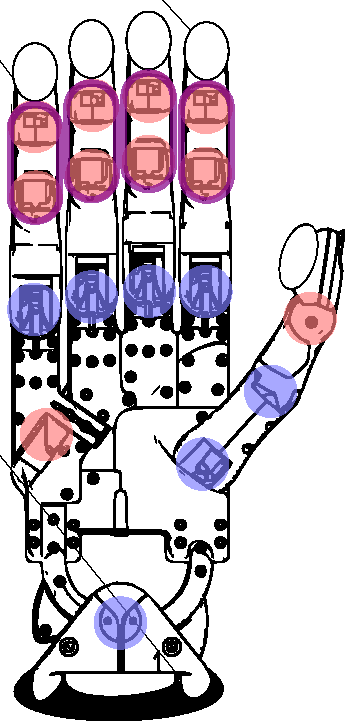
\includegraphics[height=\textwidth]{chapters/system-setup/fig/robot-hand-skeleton-coupled.pdf}
		\caption{\gls{sdh} with joints color coded depending on the degrees of freedom. The total number of degrees of freedom can here be seen as \num{24}. This figure is based on~\cite{svg-robot-hand}.}
		\label{fig:robot-hand-skeleton}
	\end{subfigure}
	\hfill
	\begin{subfigure}[b]{0.48\textwidth}
		\centering
		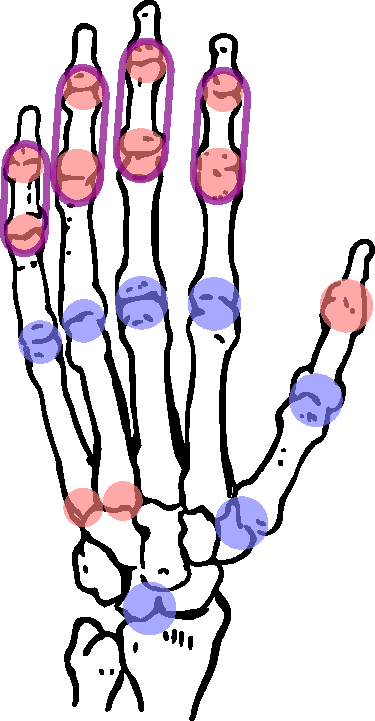
\includegraphics[height=\textwidth]{chapters/system-setup/fig/human-skeleton-hand-coupled.pdf}
		\caption{\gls{sdh} with joints color coded depending on the degrees of freedom. The total number of degrees of freedom can here be seen as \num{25}~\cite{design-and-development-of-a-bilateral-therapeutic-hand-device-for-stroke-rehabilitation}. This figure is based on~\cite{svg-skeleton-hand}.}
		\label{fig:human-hand-skeleton}
	\end{subfigure}
	\caption{The \gls{sdh} and a human hand red here marks a joint with \num{1} degree of freedom, while blue marks a joint with \num{2}.}
	\label{fig:hands-dof}
\end{figure}

The hand's geometry is modeled using a combination of standard shapes and custom-designed components. For example, the finger joints are modeled using a series of cylinders and spheres, which are connected by virtual tendons to simulate the motion of the real-world hand. The tactile sensors on the simulated hand, at the writing of this thesis, are purely aesthetical as representative simulated tactile sensors are yet to be supported as a standard component. To generate representative tactile data additional software is therefore required. The tactile sensors can be seen in \figref{fig:robot-hand-skeleton} as the ellipsoids mounted at each fingertip. \medskip

Multiple hand configurations are available including a left hand, right hand, and both configurations mounted on \gls{ur} manipulators~\cite{shadow-hand-configurations}. The configuration chosen for this project is a Shadow Dexterous right hand without being mounted on a manipulator.~\figref{fig:simulated-robot-hand} shows the \gls{cad} model of the \gls{sdh} in simulation.

\begin{figure}[h]
	\begin{small}
		\begin{center}
			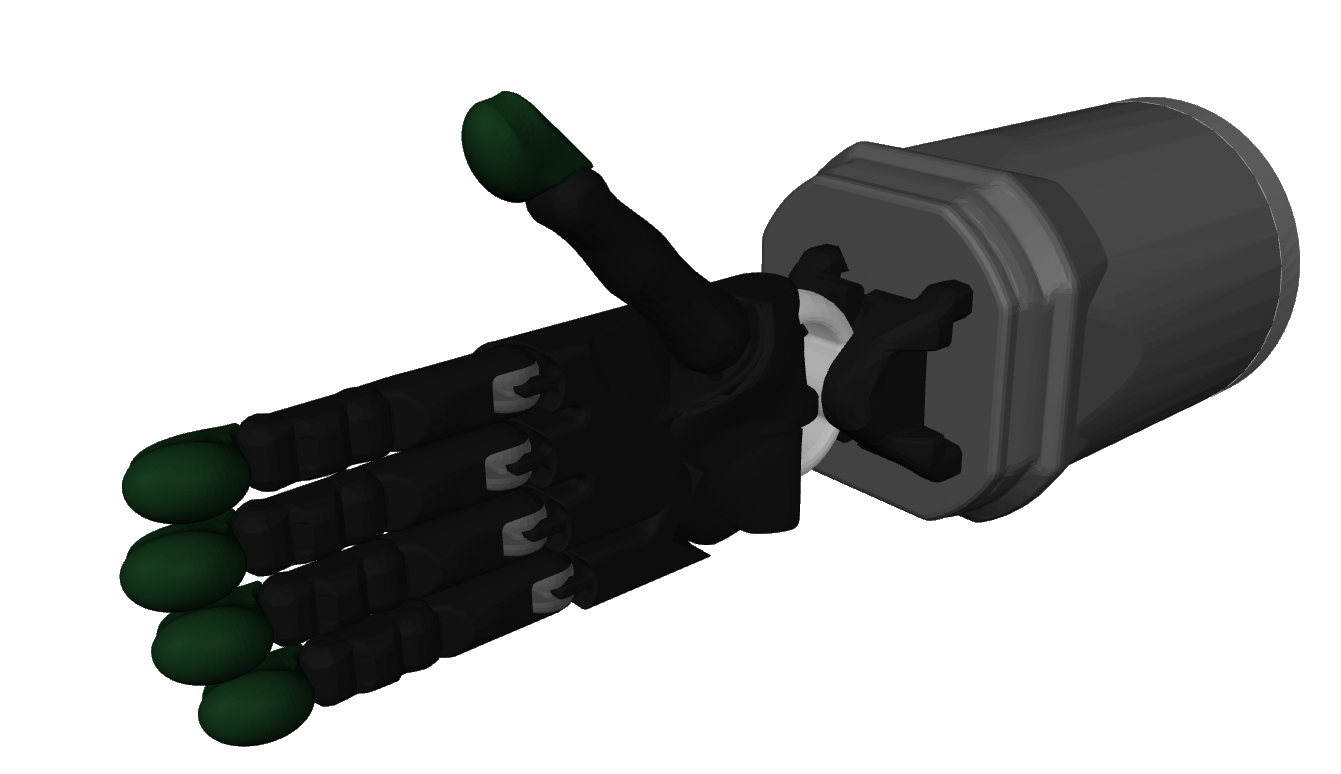
\includegraphics[width=0.5\textwidth]{chapters/system-setup/fig/simulation-robot-hand.png}
		\end{center}
		\caption{A cutout of the simulated \gls{sdh}.}
		\label{fig:simulated-robot-hand}
	\end{small}
\end{figure}

\section{Software Setup}\label{sec:system-setup-software-setup}

The software for this project consists of two parts the software provided and the software produced.

\subsection{Provided Software}\label{sec:system-setup-simulation-setup-provided}

The simulation environment is shipped in a custom Ubuntu-based docker container~\cite{docker, ubuntu-docker-image} with the necessary libraries to communicate and develop applications on the simulated as well as the physical hand, wrapped within a catkin workspace~\cite{catkin}. Additionally, the container comes with common-use libraries for Python and C++ development in \gls{ros} including \texttt{numpy}\cite{numpy}, \texttt{OpenCV}~\cite{opencv} and \texttt{dynamic\_reconfiguration}~\cite{dynamic-reconfiguration}. The development environment can be seen illustrated in \figref{fig:package-diagram}. The communication between the provided \gls{ros} packages and the Gazebo simulator is achieved through the \gls{ros}-Gazebo framework. 

\begin{figure}[!h]
	\begin{small}
		\begin{center}
			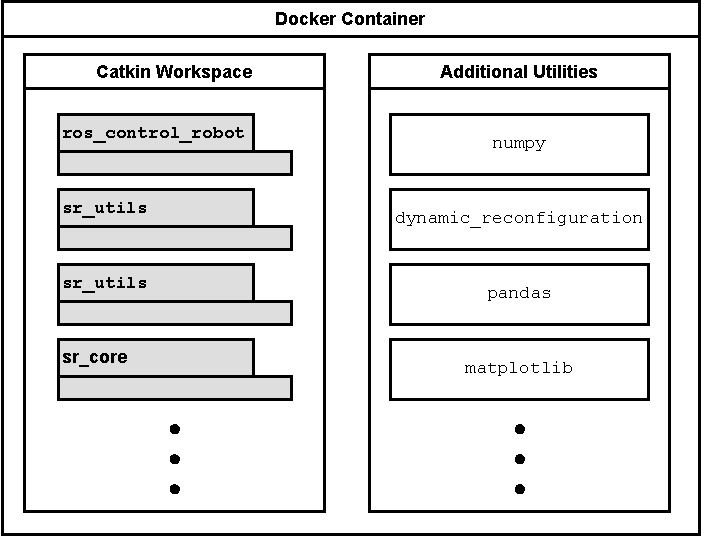
\includegraphics[width=0.5\textwidth]{chapters/system-setup/fig/init-package-diagram.pdf}
		\end{center}
		\caption{The boxes marked with grey are \gls{ros} packages, while the white are modules.}
		\label{fig:package-diagram}
	\end{small}
\end{figure}

When communicating with the \gls{sdh}, the primary interface provided is the hand commander i.e. \texttt{SrHandCommander} which enables functionalities such as retrieving the current state of the hand, executing given path plans etc. To plan and execute a high-resolution path \mvar{\mat{Q}_{\text{full}}\inR{m\times 24}}, where \mvar{m} is the number of joint configurations and \num{24} is the number of joints in the hand, a sequence of waypoints \mat{Q} form a low-resolution path of \mvar{\vec{q}_i = \rvec{q_0,\vsep q_1,\vsep \dots,\vsep q_n}^\T\inR{24}} where \mvar{i \in \{0,1,\dots,m_w\}} with \mvar{m_w} being the number of waypoints. \mat{Q} can thus be written as
\begin{equation}\label{eq:waypoint-path-matrix}
	\mat{Q} = 
		\left[\begin{array}{ccc}
			\vec{q}_1^\T \\
			\vec{q}_1^\T \\
			\vdots \\
			\vec{q}_{m_w}^\T
		\end{array}\right] \inR{m_w \times 24}.
\end{equation}

\texttt{SrHandCommander} parses the path to the \texttt{move\_group} handled by MoveIt~\cite{reducing-the-barrier-to-entry-of-complex-robotic-software:-a-moveit!-case-study}. After receiving the plan, MoveIt first checks the validity of the start and goal states concerning the robot's joint limits, collision constraints, and other constraints like self-collision avoidance. This helps to ensure that the planned path is feasible and safe for the robot to execute. Once validated, the validated path \mvar{\mat{Q}_{\text{valid}}\inR{m_q\times 24}} is parsed to \gls{ompl}~\cite{the-open-motion-planning-library} where a safe high-resolution path is built using some chosen sample-based single- or multi-query path planning method. Some examples of these methods include \gls{prm}, \gls{fmt} and \gls{rrt}-Connect, the last of which is the default used in the provided software and the one chosen for this project. To execute the path the development environment provides \texttt{SrJointPositionController} i.e. a joint space position controller by default, which is the one chosen for this project. \medskip

The controller is built using the \texttt{ros\_control}~\cite{ros-control} framework. The \texttt{ros\_control} package provides a hardware-agnostic interface, to enable the same controllers on multiple different robotics platforms, along with the same controller being applicable on real hardware as well as simulated hardware. Finally, the hardware interface communicates with a \num{20} \gls{pid} controllers, one for each independent joint to ensure control. The software architecture for communicating with the robotic hand can be seen in \figref{fig:hand-communication-architecture}, which was inspired by figures from~\cite{shadow-robotics-control-description,shadow-robotics-firmware,shadow-robotics-controlling-the-hand}.
\begin{figure}[!h]
		\begin{center}
			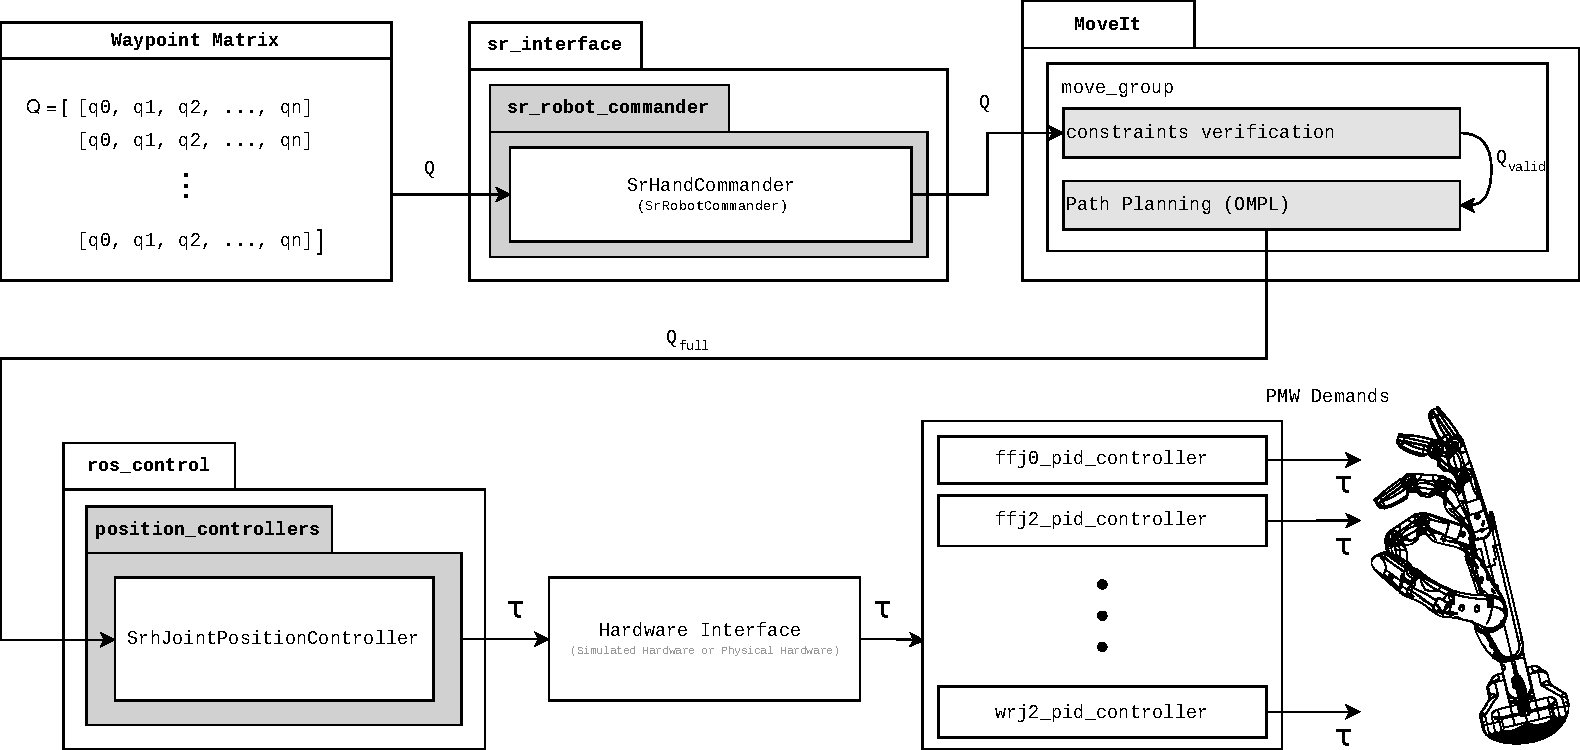
\includegraphics[width=\textwidth]{chapters/system-setup/fig/system-communication-scheme.pdf}
		\end{center}
		\caption{Diagram showing the communication and control flow of interacting with the \gls{sdh}.}
		\label{fig:hand-communication-architecture}
\end{figure}

When executing an example path~\figref{fig:coupling-and-planning-graph} shows joint angles during execution on the simulated hand throughout \SI{15}{\second}. The path here consists of five waypoints for \texttt{FFJ2} and \texttt{FFJ3}, whereas none is set for \texttt{FFJ1}. This is to demonstrate the coupling as \texttt{FFJ1} still follows the motion of \texttt{FFj2} even though no motion is commanded.

\begin{figure}[!h]
		\begin{center}
			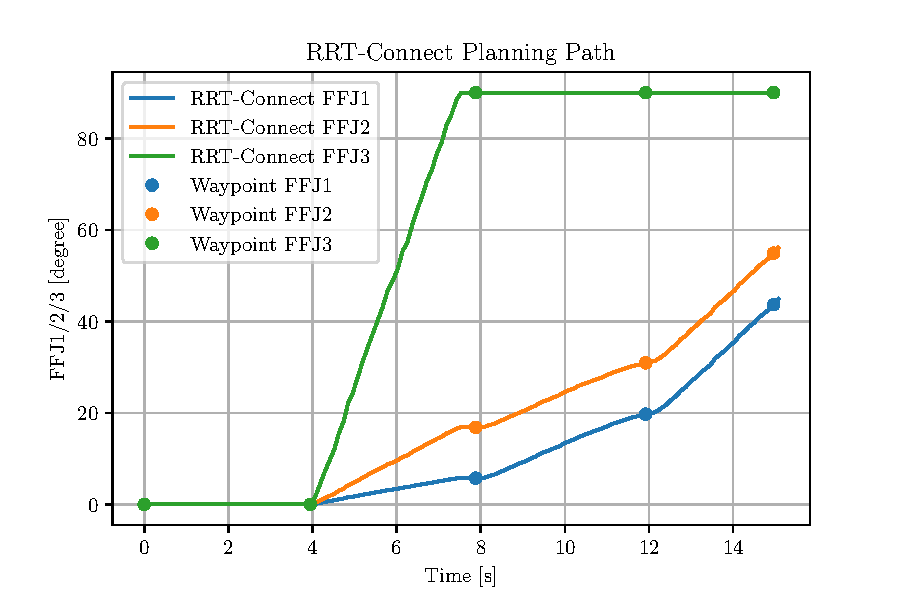
\includegraphics[width=0.6\textwidth]{chapters/system-setup/fig/q-angles.pdf}
		\end{center}
		\caption{Showing the joint trajectory of the first finger's joints \texttt{FFJ1} to \texttt{FFJ3}, where the coupling between \texttt{FFJ1} and \texttt{FFJ2} is shown.}
		\label{fig:coupling-and-planning-graph}
\end{figure}

\subsection{Produced Software}\label{sec:system-setup-simulation-setup-produced}

To execute this project, software was developed to communicate with and extract data from the simulated \gls{sdh}. 
The software is structured semantically in a similar way as the hand itself, as a \texttt{ShadowHand} contains five fingers, each labeled as one of \texttt{TH},\texttt{FF},\texttt{MF},\texttt{RF} or \texttt{LF} and a \texttt{ShadowWrist}~\ref{app:joint-abbreviations}. 
Each finger is equipped with a reader that samples the tactile data provided by Gazebo's physics engine at \SI{100}{\hertz}. This wrapper is written to an easy-to-use interface to the hand which provides reliable bookkeeping of sensor data. The structure can be seen illustrated in~\figref{fig:produced-software}.
This code is provided in a \gls{ros} package \texttt{shadow\_hand} at~\cite{in-hand-pose-estimation-repo}. 
Additionally, custom tools for easy launching and execution of experiments with live plotting of tactile data are provided with additional utilities such as base64 encoding and decoding at \texttt{ros\_utils}~\cite{ros-utils-repo}.

\begin{figure}[!h]
	\begin{center}
		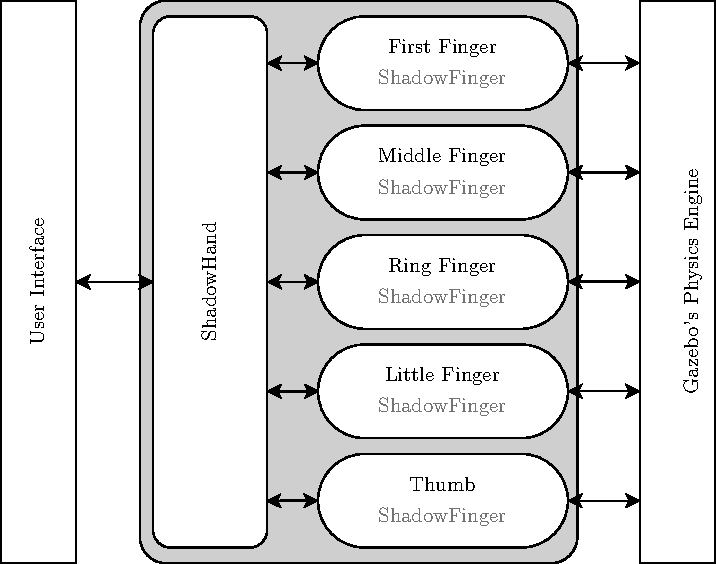
\includegraphics[width=0.6\textwidth]{chapters/system-setup/fig/produced-software-diagram(6).pdf}
	\end{center}
	\caption{Produced software architecture showing the wrapper and API structure.}
	\label{fig:produced-software}
\end{figure}
